%Lualatex+needs P22-Underground-Reg.ttf
\documentclass[
coverheight=9in,
coverwidth=6in,
spinewidth=0.4in,
bleedwidth=.125in,
marklength=0in,
markcolor=black]{bookcover}

\usepackage{xcolor}
\usepackage{background}
\usepackage{blindtext}
\usepackage{fontspec}

\setmainfont{P22UndergroundCYBookSC}

\newbookcoverpart{pfront}{
\setpartposx{\marklength+\bleedwidth+\spinewidth+\coverwidth+10mm}
\setpartposy{\marklength+\bleedwidth+10mm}\setpartheight{\coverheight-20mm}
\setpartwidth{\coverwidth-20mm}
\settrimmedpart{0mm}{0mm}{0pt}{0pt}
}

\newbookcoverpart{pback}{
\setpartposx{\marklength+\bleedwidth+10mm}
\setpartposy{\marklength+\bleedwidth+10mm}\setpartheight{\coverheight-20mm}
\setpartwidth{\coverwidth-20mm}
\settrimmedpart{0mm}{0mm}{0pt}{0pt}
}

\definecolor{top}{HTML}{002060}
\definecolor{bottom}{HTML}{0000CC}
\definecolor{line}{HTML}{2b123e}

\usetikzlibrary{calc}
\backgroundsetup{
scale=1,
angle=0,
opacity=1,
contents={
\begin{tikzpicture}
    \path [top color =top,bottom color = bottom] (current page.south west)rectangle (current page.north east);
    \path [top color =line,bottom color = line] ($(current page.south west)+(0 in,2.8 in)$)rectangle ($(current page.south east)+(0 in, 2.25 in)$);
    \end{tikzpicture}}}
    


\begin{document}

\begin{bookcover}



\bookcovercomponent{center}{spine}
{\rotatebox[origin=c]{-90}{
\color{white}
\fontsize{18}{25}\selectfont
PIGTIKAL
}}

\bookcovercomponent{normal}{pfront}{
\vskip20mm
\begin{center}
{\color{white}\fontsize{38}{48}\selectfont
PIGTIKAL\\[-2mm]
} 
{\color{white}\fontsize{32}{48}\selectfont
puzzles in geometry\\ that  I know and love\\[20mm]}
\includegraphics[angle=180, scale=1.2]{../mppics/pic-5}
\end{center}
}

\bookcovercomponent{normal}{pfront}{
\vskip154.5mm
\begin{center}
{\color{white}\fontsize{25}{48}\selectfont
Anton  Petrunin}
\end{center}
}

\bookcovercomponent{normal}{pfront}{
\vskip183mm
\begin{flushleft} 

\includegraphics[angle=0, scale=.16]{amr-small}
\end{flushleft}
}

\bookcovercomponent{normal}{pfront}{
\vskip183mm
\begin{flushright} 
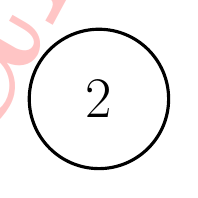
\begin{tikzpicture}
[line width=.4mm,main node/.style={circle,draw,fill=white,minimum size=17.7mm}]
\node[main node] (1) at (1,15/6) {\fontsize{20}{48}\selectfont 2};
\end{tikzpicture}
%\includegraphics[angle=0, scale=.85]{../mppics/pic-10}
\end{flushright}
}

\setmainfont{P22-Underground-Reg}

\bookcovercomponent{normal}{pfront}{
\vskip188mm
\begin{center}
{\color{white}\fontsize{12}{48}\selectfont
ASSOCIATION for MATHEMATICAL RESEARCH\\[2mm]
MONOGRAPHS: VOLUME 2}
\end{center}
}


\bookcovercomponent{normal}{pback}{
\vskip37mm
\begin{center}
{\color{white}\fontsize{14}{48}\selectfont
PIGTIKAL: puzzles in geometry that I know and love\\[1mm]
by  Anton Petrunin}
\end{center}
}

\bookcovercomponent{normal}{pback}{
\vskip154mm
\begin{center}
{\color{white}\fontsize{10}{28}\selectfont
ASSOCIATION for MATHEMATICAL RESEARCH\\[1mm]
MONOGRAPHS: VOLUME 2}
\end{center}
}

\bookcovercomponent{normal}{pback}{
\vskip181.3mm
\begin{flushleft} 

\includegraphics[angle=0, scale=.40]{amr-big}
\end{flushleft}
}


\end{bookcover}

\end{document}
